% Working paper: Foreign Gifts to Federal Officials as a Living Dataset
% Build:  pdflatex gifts_living_data && bibtex gifts_living_data && pdflatex gifts_living_data && pdflatex gifts_living_data
% Tables (tables/*.tex) and figures (figures/*.pdf) are generated by analysis/descriptives.py.

\documentclass[11pt]{article}

\usepackage[T1]{fontenc}
\usepackage{lmodern} 
\usepackage[utf8]{inputenc}
\usepackage[margin=1in]{geometry}
\usepackage{microtype}
\usepackage{graphicx}
\usepackage{booktabs}
\usepackage{array}
\usepackage{xcolor}
\usepackage{enumitem}
\usepackage{caption}
\usepackage{listings}
\usepackage{setspace}
\usepackage[authoryear,round]{natbib}
\usepackage[colorlinks=true,linkcolor=arblue,citecolor=arblue,urlcolor=arblue]{hyperref}

\definecolor{arblue}{HTML}{184F95}
\definecolor{sidebar}{HTML}{EEF4FC}
\definecolor{codebg}{HTML}{F7F7F5}

\captionsetup{font=small,labelfont=bf,labelsep=period}
\setlist{itemsep=2pt,topsep=4pt}
\setstretch{1.15}

% Annual Review-style section heads: numbered, upper case.
\makeatletter
\renewcommand\section{\@startsection{section}{1}{\z@}{-3.0ex plus -1ex minus -.2ex}{1.5ex plus .2ex}{\normalfont\large\bfseries\MakeUppercase}}
\renewcommand\subsection{\@startsection{subsection}{2}{\z@}{-2.5ex plus -1ex minus -.2ex}{1ex plus .2ex}{\normalfont\normalsize\bfseries\MakeUppercase}}
\renewcommand\subsubsection{\@startsection{subsubsection}{3}{\z@}{-2ex plus -1ex minus -.2ex}{.8ex plus .2ex}{\normalfont\normalsize\bfseries}}
\makeatother

% Sidebar box (Annual Reviews uses shaded sidebars for definitions and asides).
\newenvironment{sidebar}[1]
  {\par\medskip\noindent\begin{lrbox}{0}\begin{minipage}{\dimexpr\linewidth-2\fboxsep\relax}\small\textbf{\MakeUppercase{#1}}\par\smallskip}
  {\end{minipage}\end{lrbox}\colorbox{sidebar}{\usebox{0}}\par\medskip}

\lstdefinestyle{code}{basicstyle=\ttfamily\footnotesize,backgroundcolor=\color{codebg},
  frame=none,columns=fullflexible,keepspaces=true,showstringspaces=false,
  breaklines=true,aboveskip=6pt,belowskip=6pt,xleftmargin=4pt,xrightmargin=4pt}
\lstset{style=code}

\newcommand{\ngifts}{10,428}
\newcommand{\qid}[1]{\texttt{#1}}

\title{\textbf{Living Data for the Study of Diplomacy and Bureaucracy:}\\
\textbf{Foreign Gifts to U.S.\ Federal Officials, 1999--2023}}
\author{Raymond Hicks\thanks{Corresponding author: \href{mailto:arpie71@gmail.com}{arpie71@gmail.com}. Working paper; comments welcome. Code and data: the \texttt{gifts} repository. [Co-author names and affiliations to be added.]}}
\date{Working paper --- October 2026}

\begin{document}
\maketitle

\begin{abstract}
\noindent Every year the U.S.\ Department of State publishes, in the \emph{Federal Register}, a list of the gifts that foreign governments gave to federal employees: who gave what to whom, when, what it was worth, and what happened to it. The list is a rare, systematic, and official record of personal contact between foreign leaders and American officials, but as published it is a set of loosely formatted tables that do not link across years or to any other source. We describe a pipeline that turns these releases into a \emph{living dataset}: a collection that is rebuilt from source each time a new report appears, rather than frozen at the moment of a single coding effort. The pipeline downloads each report, parses its free-text fields, recovers the reporting agency, and resolves givers and recipients to Wikidata identifiers. The current release holds \ngifts{} gifts from 169 countries reported by 107 agency units. We argue that the persistent identifier is the key design choice. It turns a hard fuzzy-matching problem into an exact join with other person-level resources, such as the Comparative Legislators Database. It separates the \emph{office} from the \emph{officeholder}, so the same individual can be followed across careers. And it lets context that the gift reports never contain (later offices, education, party, family ties) be refreshed from Wikidata as those records grow. We present descriptive statistics by individual, country, branch, and giver type, and outline applications in international relations, legislative studies, and bureaucratic politics.
\end{abstract}

\medskip
\noindent\textbf{Keywords:} living data, Wikidata, foreign gifts, diplomacy, bureaucracy, record linkage, political elites

\vspace{1em}
\hrule
\vspace{1em}

\section{Introduction}

Political scientists increasingly study politicians and bureaucrats as individuals: their class backgrounds, careers, networks, and post-office trajectories \citep[e.g.,][]{carnes2023economic,lewis2008politics,teodoro2011bureaucratic}. These research programs share a practical bottleneck. Information about any given official is spread across many sources: rosters, appointment records, financial disclosures, travel logs, and news. Each source names people slightly differently and is updated on its own schedule. A researcher who wants to know whether a senator who later became Secretary of State received more foreign gifts in her second job than in her first must reconcile spellings (\emph{Hillary Rodham Clinton}, \emph{Mrs.\ Clinton}, \emph{Secretary Clinton}), separate the person from the office, and then redo the work when the next year of data arrives.

This paper presents a dataset designed around that bottleneck. Our substantive source is the annual list of \emph{Gifts to Federal Employees From Foreign Government Sources}, compiled by the Department of State's Office of the Chief of Protocol under the Foreign Gifts and Decorations Act \citep{usc7342}. Each entry records a recipient, a foreign giver, a description of the item, the date it was received, an estimated value, its disposition, and often a justification for accepting it. The records cover heads of state presenting gifts to presidents, defense ministers to combatant commanders, and intelligence services to the Central Intelligence Agency. Read together, they form one of the few official, systematic records of \emph{personal} contact between foreign governments and American officials, broken down by person and by year.

Our contribution is less the gift records themselves, which are public, than the infrastructure that makes them usable and keeps them current. We treat the collection as a \emph{living dataset}: one rebuilt from source each time a new report is published, with every derived variable reproducible from code and every judgment stored in versioned lookup files rather than in a one-off spreadsheet. Its central design choice is to tie each giver and recipient to a Wikidata identifier \citep[QID;][]{vrandecic2014wikidata}. That choice does three things at once.
\begin{enumerate}
\item \textbf{It makes merging cheap.} Many person-level datasets in political science already carry Wikidata IDs, most prominently the Comparative Legislators Database \citep[CLD;][]{gobel2022cld}. A QID turns a probabilistic name-matching exercise \citep{enamorado2019using} into an exact join.
\item \textbf{It separates office from officeholder.} The gift reports record the job a person held when they received a gift. The QID records the person. With both, one can follow an individual through Congress, the White House, the State Department, and the intelligence community, which is the variation that bureaucratic-politics theories often care about.
\item \textbf{It makes context updatable.} Wikidata's statements about a person's positions, education, party, and family keep growing after a gift is recorded. A living dataset can re-query those statements at each release, so covariates that a static file would freeze stay current.
\end{enumerate}

The rest of the paper is organized as follows. Section~\ref{sec:living} defines living data and why it matters for merging and updating. Section~\ref{sec:source} describes the source. Section~\ref{sec:pipeline} details the pipeline, and Section~\ref{sec:desc} presents descriptive statistics for individuals, countries, and branches. Sections~\ref{sec:link}--\ref{sec:context} develop the three advantages above: linkage, office versus officeholder, and automatic tracking of diplomatic contact. Section~\ref{sec:apps} sketches applications and the planned interactive application, and Section~\ref{sec:limits} discusses limitations.

\section{What Is a Living Dataset?}\label{sec:living}

\begin{sidebar}{Living dataset}
A \textbf{living dataset} is a continuously updating collection of data that evolves over time rather than remaining frozen in a static state. Concretely, (\emph{a}) it is rebuilt from primary sources by code whenever those sources change; (\emph{b}) human judgments (for example, ``this \emph{Abdullah} is \qid{Q57464}'') are stored as data in versioned lookup tables, so they persist across rebuilds instead of being redone; (\emph{c}) entities are keyed by persistent identifiers maintained outside the project, so linked attributes can be refreshed; and (\emph{d}) each release is reproducible, so a result can be traced to a specific version of sources, lookups, and code.
\end{sidebar}

Most datasets in political science are \emph{static}: a team codes a population over a fixed window, deposits a file, and moves on. Static datasets are valuable and often superb, but they carry two familiar costs.

\paragraph{Static data are hard to merge.} A dataset built around names, or around project-specific numeric codes, can be joined to another only through a crosswalk that someone must build. For countries this problem is largely solved by shared code systems and the tools that translate among them \citep{arelbundock2018countrycode}. For individuals it is not. Names are transliterated in many ways (the lookup file maps eleven distinct name strings, among them \emph{Abdelazia}, \emph{Abdelkaziz}, and \emph{Bonteflika}, to Abdelaziz Bouteflika's single QID), titles are folded into names, and the same person appears under different offices. Researchers therefore fall back on fuzzy or probabilistic record linkage \citep{enamorado2019using}. That is feasible but costly, and every research team repeats it with slightly different results.

\paragraph{Static data are hard to update.} When a source adds a year, a static dataset either goes out of date or must be reconstructed, often by different people with different rules. The cleaning decisions embedded in the original release (which rows were dropped, how ambiguous names were resolved) are frequently lost. The transparency and replication literature has long noted this problem \citep{king1995replication,lupia2014openness}. Event datasets such as GDELT \citep{leetaru2013gdelt} show the opposite pole: fully automated and continuously updated, but with limited human verification of who the actors are.

A living dataset sits between these poles. Updating is routine because the pipeline, not a person, does the repetitive work. Human verification is cumulative because it is stored in lookup files the pipeline consults on every run. Merging is cheap because entities are keyed to an external, community-maintained identifier. These features map closely onto the FAIR principles of findability, accessibility, interoperability, and reusability \citep{wilkinson2016fair}. The persistent identifier is what makes the data interoperable.

The gift reports suit this model particularly well. They arrive on a predictable annual cycle, roughly a year after the calendar year they cover: the report for calendar year 2024 appeared on January 29, 2026 \citep{fr2026gifts}. Their format drifts from year to year, but not by much. And most of their actors are exactly the kind of internationally prominent people Wikidata describes well.

\section{The Source: Foreign Gift Reports}\label{sec:source}

The U.S.\ Constitution's foreign emoluments clause bars federal officers from accepting any ``present'' from a foreign state without the consent of Congress. The Foreign Gifts and Decorations Act of 1966, codified at 5 U.S.C.\ \S\,7342, supplies that consent in a structured form. Employees may accept gifts of ``minimal value'' (a threshold the General Services Administration revises every three years to track the consumer price index: \$390 for 2017--2019, \$415 for 2020--2022, and \$480 for 2023--2025; \citealt{gsa2023minimal}). Gifts above the threshold may be accepted when refusing would ``cause offense or embarrassment or otherwise adversely affect the foreign relations of the United States,'' but they become property of the United States and must be reported. Each employing agency compiles these reports, and the State Department publishes the combined list annually. The statute's definition of ``foreign government'' includes international organizations, so the World Health Organization and NATO bodies appear as givers alongside heads of state. Agencies may also withhold the giver's identity when publishing it would harm intelligence sources (\S\,7342(f)(4)). We return to this below.

Each published entry has four fields:
\begin{itemize}
\item \textbf{Recipient}: name, title, and often the organization (``Admiral John Richardson, U.S.\ Navy, Chief of Naval Operations'');
\item \textbf{Gift}: a free-text block that packs together the description of the item, the date received, the estimated value, and the disposition (``\ldots{} Rec'd---August 28, 2002. Est.\ Value---\$1,000,000. Archives Foreign'');
\item \textbf{Giver}: honorific, name, title, and country (``His Royal Highness Prince Bandar bin Sultan, Ambassador of Saudi Arabia'');
\item \textbf{Circumstances}: the justification for acceptance (most often the non-embarrassment clause).
\end{itemize}
Entries are grouped into agency sections, such as ``The White House---Executive Office of the President,'' ``Department of the Navy,'' and ``United States Senate,'' and the grouping is itself informative. The reports are published as structured XML, which we use, though the content of each cell is free text.

\section{The Pipeline}\label{sec:pipeline}

Table~\ref{tab:pipeline} summarizes the pipeline. Each stage reads the output of the previous one, so a new annual report can be added with one download command and one rebuild.

\begin{table}[t]
\centering\small
\caption{Pipeline stages, scripts, and outputs.}\label{tab:pipeline}
\begin{tabular}{p{2.6cm}p{4.2cm}p{7.6cm}}
\toprule
Stage & Script & What it does \\
\midrule
1.\ Acquire & \texttt{download\_data.py} & Fetches the Federal Register XML for a report year (URLs kept in \texttt{files/urls.csv}); archives the XML; writes one raw CSV per year. \\
2.\ Parse & \texttt{parseandclean\_new.py} & Forward-fills recipient and giver across multi-item listings; splits the gift blob into item, receipt date, value, disposition, location; splits names from honorifics, ranks, titles, and organizations; standardizes dates. \\
3.\ Resolve & \texttt{wikifind.py}, \texttt{masterwiki\_new.csv}, \texttt{groups.csv}, \texttt{nowiki2.txt} & Searches Wikidata for unmatched names, has a human verify the candidates, and stores the verified mappings as lookup tables that every later run reuses. Resolves bare offices (``President'') to the holder in that year. \\
4.\ Enrich & \texttt{scripts/wiki\_properties.py} & Downloads selected Wikidata statements (positions held with start/end dates, citizenship, education, party, occupation, family, and so on) for every linked QID. \\
5.\ Analyze & \texttt{analysis/build\_analysis\_data.py} & Recovers the reporting agency from the XML section headings and groups agencies into branches; assigns giver country and giver type; builds person-level edge lists and a balanced country-year panel. \\
6.\ Describe & \texttt{analysis/descriptives.py} (\texttt{.do}) & Produces the tables and figures in this paper and an interactive map. \\
\bottomrule
\end{tabular}
\end{table}

\subsection{Acquisition and Parsing}

The reports are published in the \emph{Federal Register} without a dedicated landing page, so each year's XML URL is recorded once in \texttt{files/urls.csv}. The download step stores both the original XML and a raw CSV, so later stages can return to the source. Parsing is mostly regular-expression work, but three features of the source deserve mention because they recur in other government registers.

\emph{First}, multi-item listings name the recipient and giver once and leave later rows blank; forward-filling restores the pair for each item. \emph{Second}, the gift field packs several variables into one string, and the labels drift across years (``Est.\ Value---,'' ``Estimated Value:,'' ``Appraised Value''). The parser peels labeled fields off the end of the string. Where a disposition appears without a label (``\$280.\ Government Property''), the parser does not try to enumerate the open-ended set of disposition phrases. It instead reads the value expression, whose vocabulary is closed (currency amounts, ``each,'' ``approximately,'' punctuation), and treats whatever follows as the disposition. \emph{Third}, honorifics and ranks (``His Excellency,'' ``The Right Honorable,'' ``Admiral'') are split from names before matching, because they otherwise defeat any name lookup.

\subsection{Entity Resolution to Wikidata}

Name resolution is deliberately \emph{semi}-automated. For each name without a QID, a SPARQL query returns Wikidata humans whose label or alias matches. A human then confirms, rejects, or corrects the candidates. Fully automated matching is unsafe: a query for ``Qin Gang'' returns five people. Confirmed matches are written to a master lookup file (\texttt{masterwiki\_new.csv}, currently about 4,700 name-to-QID mappings). Names that are confirmed to have no Wikidata item are written to an exclusion list, so they are not searched again. Non-person givers and recipients receive explicit codes: \texttt{FAMILY} for joint gifts from a royal couple, \texttt{GROUP} for delegations, \texttt{UNCLEAR} for unresolvable cases, and \texttt{NIL} for statutory placeholders such as ``5 U.S.C.\ 7342(f)(4).'' This separates ``not yet looked up'' from ``looked up and not a person,'' a distinction a living dataset needs.

Recipients recorded only by role (``President,'' ``Vice President,'' ``First Lady'') are resolved by year to the person who held the role. This is the first, simplest instance of the office/officeholder distinction we develop in Section~\ref{sec:office}.

\subsection{Recovering the Reporting Agency}

The reporting agency is not a field in the parsed data, but the XML encodes it. From 2001 onward each agency's table carries a title (\texttt{<TTITLE>Agency: Department of the Navy</TTITLE>}). In 1999 and 2000 the agency appears as a one-cell row inside a single long table. Walking the XML rows in document order assigns every gift to an agency. All \ngifts{} records receive one, under 107 distinct labels, which we group into seven branches: White House (including the Office of the Vice President and the National Security Council), Diplomatic (State, USAID), Defense (the department, the services, and combatant commands), Intelligence (CIA, ODNI, DIA), Legislative (House, Senate, GAO), Judicial, and Other executive. The agency tells us \emph{which institution} reported the gift; the recipient's QID tells us \emph{who} received it.

\subsection{Giver Country and Giver Type}

We assign each gift a giving country from the text of the giver field, which almost always names the government (``\ldots{} King of the Kingdom of Saudi Arabia''). Where the text names no country, we fall back on the giver's Wikidata country of citizenship (P27). Regime-specific Wikidata items (``Islamic Republic of Afghanistan,'' ``Great Socialist People's Libyan Arab Jamahiriya'') are folded into the continuing state, so each country keeps a single identifier and ISO~3166 code across the panel. This yields a country for 84\% of gifts. Nearly all of the rest are gifts with a withheld giver identity or gifts from international organizations, which we code as their own giver type. As a check, where both sources are available (more than 5,000 gifts), the text-based country and the Wikidata citizenship agree 99\% of the time. We also classify the giver's role from honorifics and titles: royalty, head of state or government, minister, military officer, diplomat, legislator, intelligence or security official, or international organization.

\subsection{The Annual Update Cycle}

Adding a year requires (\emph{i}) recording the new XML URL, (\emph{ii}) running the download and parse scripts, (\emph{iii}) reviewing only the names that are new to the lookup files, and (\emph{iv}) re-running enrichment and analysis. Step (\emph{iii}) is the only manual one, and its cost falls over time. Heads of state, ministers, and senior American officials recur year after year, so each annual report adds proportionally fewer unmatched names. Table~\ref{tab:overview} shows the flip side: the newest period, 2019--2023, has the lowest linkage rate because its names have had the least review. In a living dataset, linkage rates are a release-specific quantity that should rise over time. In a static file, they are a permanent property of the data.

\section{Descriptive Overview}\label{sec:desc}

\begin{table}[t]
\centering\footnotesize\setlength{\tabcolsep}{4pt}
\caption{Overview by five-year period. ``Recip./Giver linked'' is the share of gifts whose recipient or giver is resolved to a Wikidata QID. Median value excludes gifts of travel and is in nominal dollars.}\label{tab:overview}
\begin{tabular}{lrrrrrrr}
\toprule
Period & Gifts & Recipients (QID) & Givers (QID) & Countries & Recip.\ linked & Giver linked & Median value (\$) \\
\midrule
1999--2003 & 2,303 & 213 & 529 & 123 & 70\% & 81\% & 450 \\
2004--2008 & 2,285 & 230 & 617 & 138 & 81\% & 84\% & 460 \\
2009--2013 & 2,688 & 373 & 845 & 137 & 68\% & 73\% & 680 \\
2014--2018 & 2,139 & 336 & 677 & 137 & 69\% & 74\% & 650 \\
2019--2023 & 1,013 & 177 & 332 & 104 & 62\% & 62\% & 795 \\
All years & 10,428 & 1,026 & 2,361 & 169 & 71\% & 76\% & 580 \\
\bottomrule
\end{tabular}

\end{table}

\begin{figure}[t]
\centering
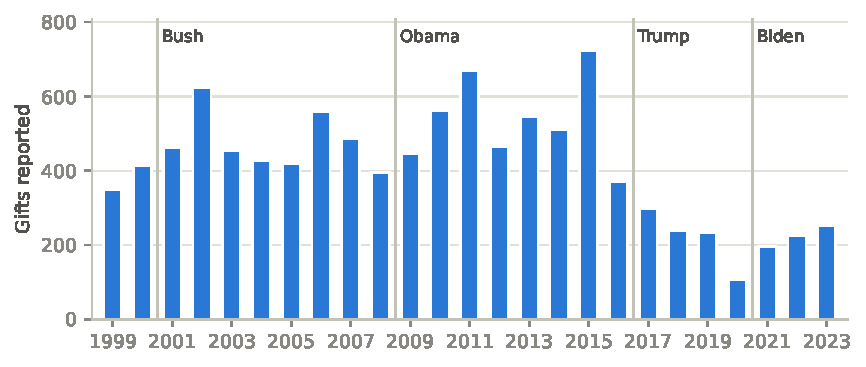
\includegraphics[width=\linewidth]{figures/fig_gifts_by_year.pdf}
\caption{Gifts reported per year (report year), 1999--2023. Vertical rules mark presidential transitions.}\label{fig:year}
\end{figure}

The current release contains \ngifts{} gifts reported between 1999 and 2023 (Table~\ref{tab:overview}). It covers 1,026 distinct recipients and 2,361 distinct givers with Wikidata identifiers, and givers from 169 countries. Seventy-one percent of gifts have a resolved recipient and 76\% a resolved giver. Ninety-four percent have a parseable dollar value; the median non-travel gift is worth about \$580, and the largest single item is a \$1,000,000 C.\,M.\ Russell painting presented by Saudi Arabia's ambassador to the First Family in 2002. About 11\% are gifts of travel or lodging, concentrated in Congress and the smaller executive agencies.

Figure~\ref{fig:year} shows the volume of reported gifts over time. Reports rose through the Obama administration, peaking at 722 in 2015, and then fell sharply: 4,291 gifts were reported for 2009--2016 against 1,549 for 2017--2023, with a low of 106 in 2020. The pandemic explains part of the 2020 trough. The 2017--2019 decline, however, began before the pandemic, and whether it reflects fewer gifts, less reporting, or changes in compilation is an open question that the data invite rather than answer. A 2024 Inspector General report found weak controls over foreign gifts \citep{gsaoig2024}. The figure also contains a measurement lesson: the 2015 spike is partly a backlog. The 2015 Senate report includes 243 gifts received years earlier, by members such as Joe Biden and Hillary Clinton while they were still senators. We therefore keep both the \emph{report year} and the \emph{receipt year} (available from the gift's date for 92\% of records). In about 5\% of records the two differ by more than a year.

\subsection{Recipients by Branch}

\begin{table}[t]
\centering\footnotesize\setlength{\tabcolsep}{4pt}
\caption{Gifts by branch of the reporting agency. ``Confidential giver'' is the share of gifts where the giver is withheld under 5 U.S.C.\ \S\,7342(f)(4). ``Travel'' is the share that are gifts of travel or lodging.}\label{tab:branch}
\begin{tabular}{lrrrrrrr}
\toprule
Branch & Gifts & Share & Agencies & Recip.\ linked & Giver linked & Confidential giver & Travel \\
\midrule
White House & 3,827 & 37\% & 16 & 84\% & 91\% & 0\% & 0\% \\
Diplomatic & 1,655 & 16\% & 9 & 76\% & 84\% & 0\% & 2\% \\
Defense & 1,890 & 18\% & 15 & 69\% & 69\% & 0\% & 3\% \\
Legislative & 1,115 & 11\% & 7 & 73\% & 90\% & 0\% & 41\% \\
Intelligence & 947 & 9\% & 4 & 35\% & 1\% & 99\% & 2\% \\
Other executive & 952 & 9\% & 55 & 46\% & 75\% & 0\% & 57\% \\
Judicial & 42 & 0\% & 1 & 83\% & 81\% & 0\% & 71\% \\
\bottomrule
\end{tabular}

\end{table}

\begin{figure}[t]
\centering
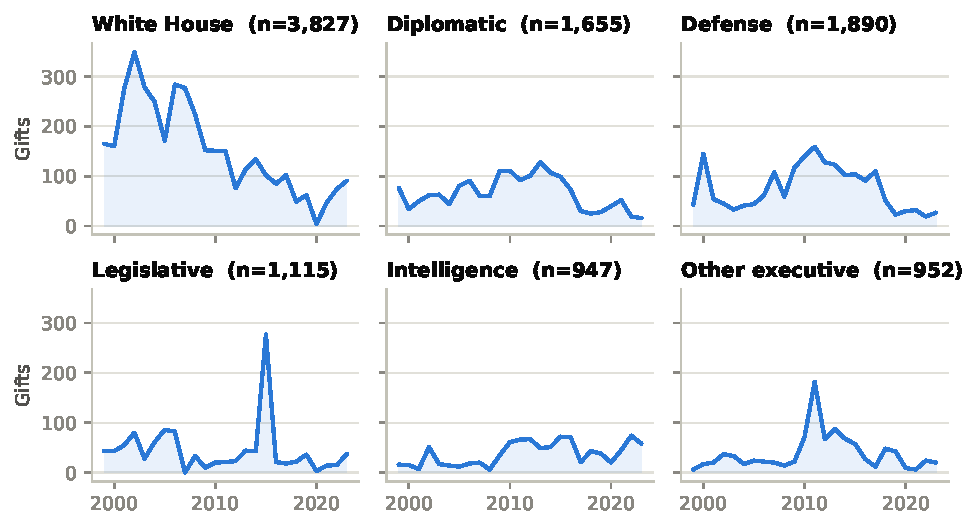
\includegraphics[width=\linewidth]{figures/fig_branch_multiples.pdf}
\caption{Gifts per year by branch of the reporting agency (report year). Panels share a y-axis. The Judicial branch (42 gifts) is omitted.}\label{fig:branch}
\end{figure}

The branch of the reporting agency structures almost everything about a gift (Table~\ref{tab:branch}, Figure~\ref{fig:branch}). The White House accounts for 37\% of gifts. These are the gifts of summit diplomacy, given overwhelmingly by heads of state and royalty and almost all resolvable to named people. Defense (18\%) and Diplomatic (16\%) agencies follow. Defense gifts flow largely from foreign military officers to American commanders, and their volume tracks the wars in Iraq and Afghanistan, peaking around 2011. Congress (11\%) is distinctive in that 41\% of its reported gifts are travel, which reflects congressional delegations. The intelligence community (9\%) is almost entirely opaque: 99\% of its gifts list the giver only as ``5 U.S.C.\ 7342(f)(4),'' and only 35\% of its recipients are named. This is a substantive feature, not a parsing failure, and analysts should treat intelligence gifts as an \emph{institution-level} rather than a person-level record.

\subsection{Givers and Recipients by Level}

\begin{figure}[t]
\centering
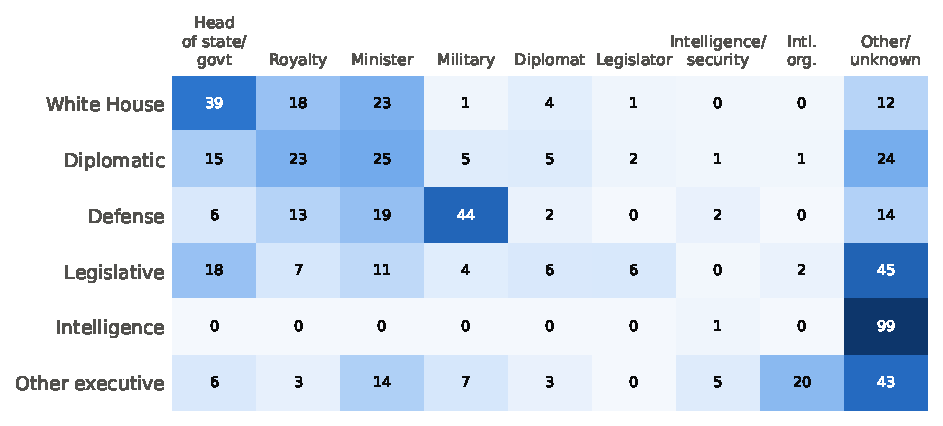
\includegraphics[width=\linewidth]{figures/fig_role_branch.pdf}
\caption{Who gives to whom. Cells show the percentage of each recipient branch's gifts that come from each type of giver (rows sum to 100). Giver type is coded from honorifics and titles.}\label{fig:rolebranch}
\end{figure}

Figure~\ref{fig:rolebranch} cross-tabulates the level of the giver against the branch of the recipient. The diagonal structure is striking: foreign governments match the rank and function of their counterpart. Heads of state and government account for 40\% of gifts to the White House, and royalty for another 18\%. Military officers account for 44\% of gifts to Defense. Ministers are spread across the White House, State, and Defense, consistent with their role as counterparts to cabinet secretaries. Foreign legislators are a small share of givers even to Congress. Most gifts to Congress come from heads of government, ministers, and unspecified officials, many of them hosting congressional delegations abroad. The pattern suggests that the gift record captures \emph{protocol-matched} contact: each tier of the U.S.\ government has a characteristic foreign counterpart. This is the kind of relationship that a network view of the data (Section~\ref{sec:apps}) makes visible.

\subsection{Individuals}

\begin{table}[t]
\centering\footnotesize
\caption{Top recipients by number of gifts (Wikidata-linked). Value is the nominal sum of estimated values. Branch lists every branch under which the person received gifts.}\label{tab:recips}
\begin{tabular}{lllrrr}
\toprule
Name & Branch & Wikidata & Gifts & Years & Value (\$) \\
\midrule
George W. Bush & White House & Q207 & 888 & 2001--2008 & 1,107,429 \\
Barack Obama & White House, Legislative & Q76 & 482 & 2005--2016 & 2,031,573 \\
Laura Bush & White House & Q152019 & 445 & 2001--2008 & 470,173 \\
Hillary Clinton & White House, Diplomatic, Legislative & Q6294 & 298 & 1999--2015 & 1,278,972 \\
Condoleezza Rice & White House, Diplomatic & Q47216 & 246 & 2001--2008 & 1,265,892 \\
Joe Biden & White House, Legislative & Q6279 & 229 & 2000--2023 & 554,104 \\
John Kerry & Diplomatic, Legislative & Q22316 & 165 & 2001--2023 & 338,428 \\
Michelle Obama & White House & Q13133 & 154 & 2009--2016 & 1,847,616 \\
Bill Clinton & White House, Diplomatic & Q1124 & 151 & 1999--2010 & 222,532 \\
Colin Powell & Diplomatic & Q150851 & 150 & 2001--2016 & 183,094 \\
Dick Cheney & White House & Q48259 & 101 & 2004--2008 & 210,735 \\
Donald Rumsfeld & Defense & Q184650 & 88 & 2001--2006 & 151,621 \\
John Owen Brennan & White House, Intelligence & Q984191 & 83 & 2009--2016 & 133,782 \\
Donald Trump & White House & Q22686 & 82 & 2017--2019 & 230,192 \\
Robert Gates & Defense & Q212979 & 79 & 2006--2011 & 64,040 \\
\bottomrule
\end{tabular}

\end{table}

\begin{table}[t]
\centering\footnotesize
\caption{Top givers by number of gifts (Wikidata-linked).}\label{tab:givers}
\begin{tabular}{lllrrr}
\toprule
Name & Country & Wikidata & Gifts & Years & Value (\$) \\
\midrule
Abdullah II of Jordan & Jordan & Q57464 & 210 & 2000--2023 & 332,229 \\
Abdullah of Saudi Arabia & Saudi Arabia & Q57298 & 188 & 2000--2018 & 5,903,000 \\
Hamid Karzai & Afghanistan & Q43944 & 160 & 2002--2020 & 276,648 \\
Hamad bin Ali Al Attiyah & Qatar & Q21004768 & 129 & 2001--2018 & 380,328 \\
Silvio Berlusconi & Italy & Q11860 & 124 & 2001--2015 & 404,420 \\
Hassanal Bolkiah I of Brunei & Brunei & Q57327 & 96 & 1999--2023 & 118,589 \\
Mohammed VI of Morocco & Morocco & Q57553 & 69 & 1999--2016 & 291,119 \\
Mohamed Hussein Tantawi & Egypt & Q45917 & 64 & 1999--2011 & 40,210 \\
Salman bin Hamad, Crown Prince of Bahrain & Bahrain & Q58140 & 63 & 2000--2023 & 140,156 \\
Ali Bin Fetais Al-Marri & Qatar & Q55081149 & 61 & 2006--2019 & 190,397 \\
Sabah Al-Ahmad Al-Jaber Al-Sabah & Kuwait & Q57555 & 53 & 2001--2019 & 171,860 \\
Pervez Musharraf & Pakistan & Q40495 & 50 & 2000--2015 & 33,572 \\
Abd al-Aziz Boutafliqa & Algeria & Q57308 & 50 & 2000--2016 & 41,882 \\
Islam Karimov & Uzbekistan & Q57558 & 46 & 1999--2015 & 29,754 \\
World Health Organization & (intl. org.) & Q7817 & 45 & 2007--2019 & 103,219 \\
\bottomrule
\end{tabular}

\end{table}

Tables~\ref{tab:recips} and~\ref{tab:givers} list the most frequent recipients and givers. Presidents and their spouses dominate the recipient list; George W.\ Bush alone received 888 reported gifts. Secretaries of State come next. The giver list is a roster of long-serving leaders, above all Gulf and Middle Eastern monarchs: Abdullah II of Jordan (210 gifts, 2000--2023), King Abdullah of Saudi Arabia, Hamid Karzai, and Qatar's Hamad bin Ali Al Attiyah. Long tenure means many opportunities to give. The values are highly skewed. King Abdullah's 188 gifts total \$5.9 million, much of it in jewelry sets presented to first ladies, cabinet officials, and their spouses, while Brunei's sultan gave 96 gifts worth about \$120,000 in total.

\subsection{Countries}

\begin{table}[t]
\centering\footnotesize
\caption{Top giving countries. ``Active years'' is the number of report years (of 25) with at least one gift. ``Main recipient branch'' is the modal branch.}\label{tab:countries}
\begin{tabular}{llrrrrl}
\toprule
Country & ISO3 & Gifts & Active years & Recipients & Value (\$) & Main recipient branch \\
\midrule
Saudi Arabia & SAU & 477 & 25 & 131 & 8,554,042 & White House \\
Qatar & QAT & 438 & 24 & 124 & 1,343,133 & Defense \\
Afghanistan & AFG & 383 & 22 & 122 & 539,854 & Defense \\
Jordan & JOR & 337 & 25 & 88 & 430,180 & White House \\
China & CHN & 293 & 25 & 105 & 334,720 & White House \\
United Arab Emirates & ARE & 278 & 25 & 93 & 583,853 & Defense \\
Pakistan & PAK & 254 & 25 & 105 & 213,268 & Legislative \\
Italy & ITA & 242 & 23 & 70 & 516,856 & White House \\
Bahrain & BHR & 234 & 25 & 76 & 530,229 & Diplomatic \\
Iraq & IRQ & 211 & 19 & 87 & 257,971 & Defense \\
Japan & JPN & 192 & 24 & 68 & 232,363 & White House \\
Kuwait & KWT & 190 & 23 & 58 & 372,511 & Defense \\
Egypt & EGY & 184 & 24 & 71 & 159,614 & Defense \\
South Korea & KOR & 183 & 25 & 71 & 170,893 & White House \\
Russia & RUS & 178 & 21 & 52 & 220,494 & White House \\
India & IND & 160 & 24 & 59 & 209,718 & White House \\
Turkey & TUR & 153 & 19 & 47 & 103,373 & White House \\
France & FRA & 148 & 22 & 48 & 220,340 & White House \\
Brunei & BRN & 140 & 19 & 32 & 422,239 & White House \\
Mexico & MEX & 136 & 21 & 47 & 103,790 & White House \\
\bottomrule
\end{tabular}

\end{table}

\begin{figure}[t]
\centering
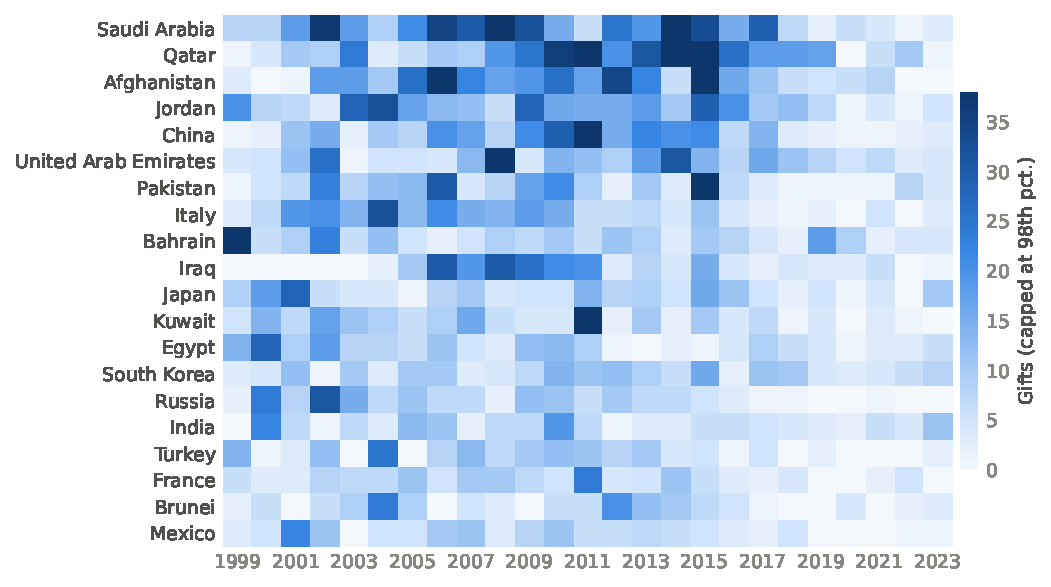
\includegraphics[width=\linewidth]{figures/fig_country_heatmap.pdf}
\caption{Gifts per year from the twenty most frequent giving countries. Darker cells mean more gifts. The scale is capped at the 98th percentile so a few extreme cells do not wash out the rest.}\label{fig:heatmap}
\end{figure}

Table~\ref{tab:countries} and Figure~\ref{fig:heatmap} aggregate gifts to the country level. Saudi Arabia (477 gifts, \$8.6 million), Qatar, Afghanistan, Jordan, China, and the United Arab Emirates lead. Gulf states are heavily overrepresented relative to their population or economic size, consistent with a gift-giving diplomatic culture and close security ties. The heatmap shows that country-level gift flows carry the imprint of events: Afghanistan and Iraq rise and fall with U.S.\ deployments, Qatar's gifts climb through the 2010s as Al Udeid became the hub of U.S.\ air operations, and Russia's are concentrated in the early 2000s and nearly vanish after 2016. Only Saudi Arabia, Jordan, China, the UAE, Pakistan, Bahrain, and South Korea give in every one of the 25 years.

\section{The Wikidata Identifier as a Linking Key}\label{sec:link}

\begin{table}[t]
\centering\small
\caption{Share of Wikidata-linked recipients and givers for whom Wikidata supplies each attribute (from a snapshot of statements for all linked QIDs).}\label{tab:wdcov}
\begin{tabular}{lrr}
\toprule
Attribute (property) & Recipients (N=1,026) & Givers (N=2,361) \\
\midrule
Gender (P21) & 98\% & 84\% \\
Date of birth (P569) & 85\% & 80\% \\
Citizenship (P27) & 82\% & 80\% \\
Occupation (P106) & 91\% & 81\% \\
Position held (P39) & 59\% & 71\% \\
Educated at (P69) & 88\% & 65\% \\
Party membership (P102) & 46\% & 52\% \\
Employer (P108) & 31\% & 15\% \\
Military rank (P410) & 21\% & 15\% \\
Spouse (P26) & 14\% & 30\% \\
Child (P40) & 7\% & 19\% \\
Father (P22) & 11\% & 19\% \\
\bottomrule
\end{tabular}

\end{table}

A QID is a join key and a gateway at once. As a gateway, it connects each gift to whatever Wikidata knows about the people involved. Table~\ref{tab:wdcov} shows that, for linked recipients, Wikidata supplies gender for 98\%, occupation for 91\%, education for 88\%, date of birth for 85\%, and at least one dated position for 59\%. Coverage of givers is similar. Collecting these covariates by hand for 3,400 people in some 170 countries would be a project in itself. Through the QID they arrive with one batched API call per 50 people.

\subsection{Joining to the Comparative Legislators Database}

\begin{table}[t]
\centering\small
\caption{Recipients and givers who ever held a seat in a chamber covered by the Comparative Legislators Database, identified from Wikidata positions held (P39). These people can be joined to the CLD on \texttt{wikidataid} with no name matching.}\label{tab:cld}
\begin{tabular}{lrrrr}
\toprule
Legislature & Recipients & Gifts received & Givers & Gifts given \\
\midrule
Italy & 0 & 0 & 22 & 164 \\
Japan & 0 & 0 & 31 & 92 \\
France & 0 & 0 & 16 & 79 \\
Turkey & 0 & 0 & 16 & 72 \\
Canada & 0 & 0 & 15 & 55 \\
Ireland & 0 & 0 & 7 & 52 \\
Germany & 0 & 0 & 13 & 46 \\
Israel & 0 & 0 & 14 & 46 \\
United Kingdom & 0 & 0 & 12 & 32 \\
Czech Republic & 0 & 0 & 11 & 24 \\
Spain & 0 & 0 & 9 & 15 \\
Austria & 0 & 0 & 8 & 11 \\
Netherlands & 0 & 0 & 5 & 10 \\
United States & 247 & 2,314 & 0 & 0 \\
\bottomrule
\end{tabular}

\end{table}

The Comparative Legislators Database \citep{gobel2022cld} assembles individual-level data on more than 67,000 legislators in 16 countries and keys every legislator to both a Wikipedia page ID and a Wikidata ID. Because the CLD and our data share that key, linking them is an exact join. Table~\ref{tab:cld} shows the scale of the overlap. Two hundred forty-seven of our recipients served in the U.S.\ House or Senate at some point, and they account for 2,314 gifts, including gifts received \emph{after} leaving Congress, as Secretaries of State, Vice Presidents, or CIA directors. On the giver side, 179 foreign officials sat in a CLD chamber, led by members of the Italian Chamber of Deputies (22 people, 164 gifts), the Japanese House of Representatives (31 people, 92 gifts), and the French National Assembly. Once joined, a researcher has, for each legislator-recipient, the CLD's political histories, committee and office records, and Wikipedia traffic, alongside the gifts that person received. With the CLD's R interface \citep{legislatoR}, the join takes a few lines:

\begin{lstlisting}[language=R,caption={Joining gift recipients to the CLD (R).}]
library(legislatoR); library(dplyr)
gifts  <- read.csv("analysis/output/gifts_analysis.csv")
house  <- get_core(legislature = "usa_house")      # one row per legislator
senate <- get_core(legislature = "usa_senate")
congress <- bind_rows(house, senate) |> distinct(wikidataid, .keep_all = TRUE)

linked <- gifts |>
  inner_join(congress, by = c("recip_wiki" = "wikidataid"))   # exact key, no fuzzy match
\end{lstlisting}

The same logic extends beyond the CLD. Any dataset that carries QIDs, or that can be crosswalked to them once, becomes joinable. For leaders, the giving side of the gift relationship could be matched to leader-level resources such as Archigos \citep{goemans2009archigos} and LEAD \citep{ellis2015lead}: the match is done once, at the level of a few hundred heads of state, and the QID then carries it to every gift. Donor and ideology data such as DIME \citep{bonica2014mapping} could be crosswalked the same way for American recipients. For countries, the ISO codes stored on Wikidata country items connect the country-year panel to standard cross-national data through existing converters \citep{arelbundock2018countrycode}.

\subsection{Why the Key Matters for Living Data}

Persistent identifiers also make the link durable. If our data and the CLD both update, the join still works, because neither project's internal row numbers or name spellings matter. By contrast, a crosswalk built between two static files on names breaks as soon as either file is revised. The QID moves the work of maintaining identity out of individual research projects and into a shared, openly edited resource. When a Wikidata editor merges two duplicate items for the same person, every project keyed to that person benefits.

\section{Office Versus Officeholder}\label{sec:office}

\begin{table}[t]
\centering\footnotesize
\caption{Recipients who received gifts under more than one branch, with the sequence of branches and the years in which gifts were received. Fifty-three recipients meet this criterion; the fifteen with the most gifts are shown.}\label{tab:careers}
\begin{tabular}{llrp{0.55\linewidth}}
\toprule
Name & Wikidata & Gifts & Sequence of reporting branches (years received) \\
\midrule
Barack Obama & Q76 & 482 & Legislative (2005--2008) $\rightarrow$ White House (2009--2016) \\
Hillary Clinton & Q6294 & 298 & White House (1998--2000) $\rightarrow$ Legislative (2002--2007) $\rightarrow$ Diplomatic (2009--2013) \\
Condoleezza Rice & Q47216 & 246 & White House (2001--2004) $\rightarrow$ Diplomatic (2005--2008) \\
Joe Biden & Q6279 & 229 & Legislative (2000--2009) $\rightarrow$ White House (2009--2023) \\
John Kerry & Q22316 & 165 & Legislative (2001--2012) $\rightarrow$ Diplomatic (2013--2023) \\
Bill Clinton & Q1124 & 151 & White House (1998--2000) $\rightarrow$ Diplomatic (2009--2010) \\
John Owen Brennan & Q984191 & 83 & White House (2009--2012) $\rightarrow$ Intelligence (2013--2017) \\
David Petraeus & Q28591 & 49 & Defense (2009--2010) $\rightarrow$ Intelligence (2011--2012) \\
Leon Panetta & Q244631 & 49 & Intelligence (2009--2011) $\rightarrow$ Defense (2011--2012) \\
Mike Pompeo & Q473239 & 47 & Intelligence (2017--2018) $\rightarrow$ Diplomatic (2018--2020) \\
Antony Blinken & Q7821917 & 38 & Legislative (2002--2009) $\rightarrow$ White House (2012--2013) $\rightarrow$ Diplomatic (2015--2023) \\
Chuck Hagel & Q381670 & 36 & Legislative (2000--2006) $\rightarrow$ Defense (2012--2015) \\
William Joseph Burns & Q1276563 & 36 & Diplomatic (2004--2014) $\rightarrow$ Intelligence (2021--2023) \\
David S. Cohen & Q20067627 & 23 & Other executive (2010--2012) $\rightarrow$ Intelligence (2015--2022) \\
Susan Rice & Q50612 & 16 & Diplomatic (2011) $\rightarrow$ White House (2013--2015) \\
\bottomrule
\end{tabular}

\end{table}

\begin{figure}[t]
\centering
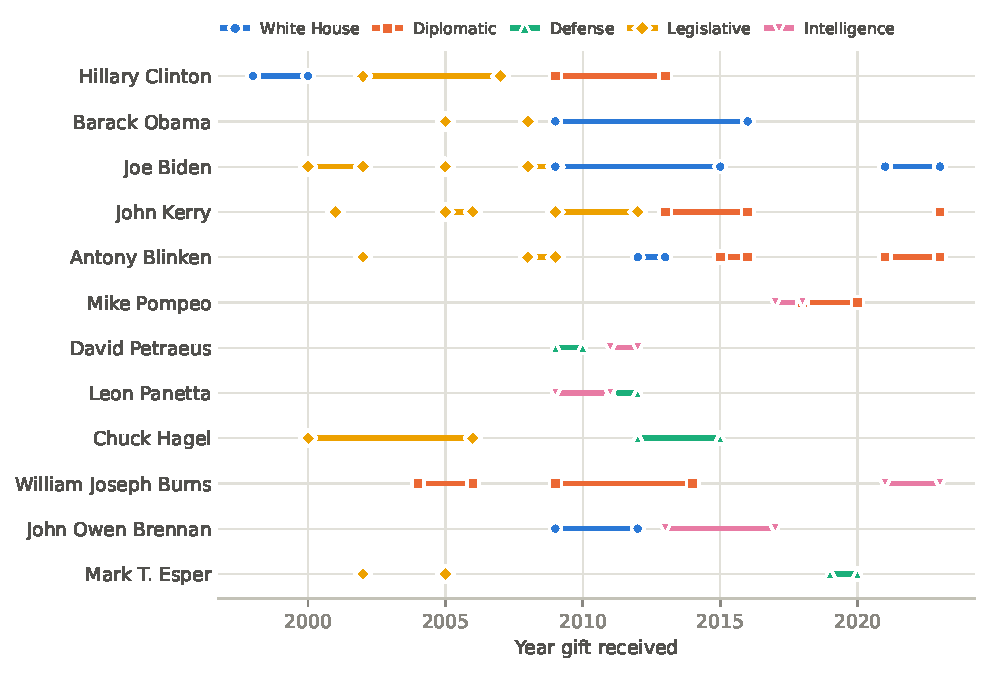
\includegraphics[width=\linewidth]{figures/fig_careers.pdf}
\caption{Careers traced through the gift record. Each row is one person (one Wikidata QID). Segments span consecutive years in which that person received gifts reported by a given branch; gaps of more than two years break a segment. Colors and marker shapes both identify the branch.}\label{fig:careers}
\end{figure}

The study of bureaucracy has long distinguished the office, with its authority, its agenda, and its foreign counterparts, from the person who occupies it, with their ambition, expertise, and networks \citep{gailmard2007slackers,lewis2008politics,teodoro2011bureaucratic}. Many administrative datasets record only the office. The gift reports record both, and the QID lets us separate them.

Table~\ref{tab:careers} and Figure~\ref{fig:careers} show what this looks like. Fifty-three recipients received gifts under more than one branch. Hillary Clinton appears as First Lady (White House, 1998--2000), as a senator (2002--2007), and as Secretary of State (2009--2013). Mike Pompeo moves from the CIA to State; Leon Panetta from the CIA to Defense; David Petraeus from Central Command to the CIA; William Burns from the State Department to the CIA; John Brennan from the White House to the CIA. Antony Blinken appears as a Senate Foreign Relations Committee staffer, as a White House national security official, and as Deputy Secretary and then Secretary of State. The office-level record (``the intelligence community reported 947 gifts'') and the person-level record (``Pompeo received 47 gifts, under two branches'') answer different questions, and the QID lets a researcher move between them.

The design supports several kinds of analysis:
\begin{itemize}
\item \textbf{Within-person comparisons across offices.} Does the same individual receive more, or more valuable, gifts after moving to a more senior or more externally facing office? Holding the person fixed isolates the effect of the office.
\item \textbf{Within-office comparisons across holders.} Do successive holders of the same post (Secretaries of State, CENTCOM commanders) attract similar gift portfolios, or do some holders carry their foreign relationships with them? A giver who presents gifts to the same American across several of that person's posts is evidence of a \emph{personal}, not institutional, tie.
\item \textbf{Revolving doors and career paths.} Movements between Congress, the executive, and the intelligence community, and on to the private sector, are central to research on capture and influence \citep{dalbo2006regulatory,blanes2012revolving}. The gift record observes the public-sector legs of these paths with exact dates.
\end{itemize}

\subsection{Wikidata Updates What the Gift Record Cannot}

The gift record observes a person only while they hold an office that receives foreign gifts. Wikidata observes the whole career and keeps observing it. Liz Cheney appears in our data in 2005 as a Principal Deputy Assistant Secretary of State and in 2008 as ``Vice President's daughter.'' Her later service in the House of Representatives (2017--2023) is absent from the gift reports but is recorded in Wikidata, with start and end dates, and arrives automatically through her QID. Mike Pompeo enters the gift record as CIA director, but Wikidata supplies the four House terms before it. For a living dataset this is the key property. Because enrichment is re-run at every release, a recipient who later becomes an ambassador, a legislator, a lobbyist, or a convicted official acquires that attribute without anyone revisiting the gift data. The query that refreshes positions for any set of people is short:

\begin{lstlisting}[caption={Positions held, with dates, for a set of recipients (SPARQL, Wikidata Query Service).}]
SELECT ?person ?personLabel ?positionLabel ?start ?end WHERE {
  VALUES ?person { wd:Q6294 wd:Q473239 wd:Q5362573 }   # Clinton, Pompeo, Liz Cheney
  ?person p:P39 ?st . ?st ps:P39 ?position .
  OPTIONAL { ?st pq:P580 ?start }  OPTIONAL { ?st pq:P582 ?end }
  SERVICE wikibase:label { bd:serviceParam wikibase:language "en". }
} ORDER BY ?person ?start
\end{lstlisting}

The same mechanism works on the giver side. Abdullah of Saudi Arabia appears in our data first as Crown Prince and First Deputy Prime Minister and later as King. Rather than re-coding each giver's title by hand, a researcher can read the giver's office at the date of the gift from Wikidata's dated P39 statements.

\section{Automatic Tracking of Diplomatic Contact}\label{sec:context}

A gift requires a meeting, or at least the delivery of a personal token from one official to another. Gift records therefore proxy \emph{personal diplomatic contact}, and because each gift carries a receipt date, the proxy is timed to the day. This complements existing measures of diplomatic ties, which typically record embassies \citep{kinne2014dependent} or leader visits \citep{lebovic2016diplomatic,malis2021state,goldsmith2021public}. Gift records reach further down the hierarchy than those measures do, to commanders, deputy secretaries, and congressional staff, and they record who met whom.

The pipeline produces this measure automatically. Each release writes a balanced country-year panel (169 countries $\times$ 25 years = 4,225 rows) with the number of gifts, total value, and number of distinct American recipients. Only 43\% of country-years record any gift, so the indicator varies a great deal both across countries and within them over time. Because the panel is keyed by ISO code, it merges directly with standard country-year data. Because it is regenerated with each release, a new year of contact appears without additional coding.

Two features make gift-based tracking especially useful for studies of particular events or relationships.
\begin{itemize}
\item \textbf{Event alignment.} With receipt dates, gifts can be aligned with independently recorded events: presidential and secretarial trips and foreign leader visits recorded by the State Department's Office of the Historian \citep{historian}, summits, arms sales, or crises. The match rate between gifts and visits is itself a validation exercise. A visit without a gift, or a gift without a recorded visit, points to an encounter that one source missed.
\item \textbf{Relevant years for a given actor.} For any person or country, the data identify the years in which contact with American officials occurred, and with whom. A researcher interested in, for example, Qatari engagement with the U.S.\ military can find the relevant years and counterparts directly, rather than combing through news archives.
\end{itemize}

\section{Applications}\label{sec:apps}

The finished data project supports research across several subfields.

\paragraph{Diplomacy and alliance politics.} Gift flows provide a person-level measure of the intensity and seniority of bilateral contact. Researchers can ask whether contact intensifies before arms sales, basing agreements, or votes in international organizations; whether it shifts with changes of government in Washington or abroad; and whether some states cultivate the military rather than civilian leaders (Figure~\ref{fig:rolebranch}).

\paragraph{Influence, emoluments, and accountability.} Gifts are the most literal form of foreign influence over officials, and gift exchange has deep roots as a mechanism of obligation \citep{mauss1990gift}. The data allow systematic study of who receives the most valuable gifts, whether value tracks policy salience, and how dispositions (retained for official display, transferred to the National Archives, purchased by the recipient) vary across agencies. Linked to lobbying and post-government employment data through QIDs, they connect foreign gift-giving to later career outcomes.

\paragraph{Legislative studies.} Through the CLD and Wikidata positions, gifts to members of Congress can be connected to committee assignments, seniority, and electoral histories. Congressional travel gifts (41\% of congressional gifts) provide a measure of foreign-funded delegation travel that can be compared with legislators' committee portfolios, in the spirit of research on informational lobbying \citep{hall2006lobbying}. On the giver side, foreign legislators identified through the CLD give a view of parliamentary diplomacy.

\paragraph{Bureaucratic politics and careers.} The office/officeholder design supports studies of political appointees versus career officials \citep{lewis2008politics}, of how ambition shapes behavior \citep{teodoro2011bureaucratic}, and of how foreign relationships accompany officials across posts. Because Wikidata keeps updating positions, the post-government careers of recipients accumulate automatically.

\paragraph{Gender and the politics of the spouse.} First ladies are among the largest recipients by value (Michelle Obama's 154 gifts total \$1.8 million), and the data distinguish gifts given to officials in their own right from gifts given to spouses and family. Combined with Wikidata's gender and family statements, the data speak to research on gendered roles in political life \citep{teele2018ties}.

\paragraph{Networks.} Each release writes a person-to-person edge list (4,195 giver--recipient pairs with counts, values, and first and last years) suitable for network analysis \citep{hafner2009network,ward2011network}. Centrality measures identify the American officials who serve as hubs of foreign contact and the foreign officials who reach across many U.S.\ institutions. Bipartite projections reveal which American offices share foreign counterparts.

\paragraph{A template for other registers.} Many governments publish gift, hospitality, and interest registers for ministers and legislators, in formats as loose as the American one. The pipeline's architecture, in which lookups are stored as data, entities are keyed by QID, and every step is rebuilt from source, transfers directly. Wikidata-keyed registers from several countries would support the first comparative study of official gift-giving.

\subsection{The Interactive Application}

We are building a Streamlit application on top of the pipeline outputs. It will have two primary views. A \emph{network view} draws the person-level edge list, filterable by year, branch, giver type, and country, with nodes linked to their Wikidata pages. A \emph{map view} renders the country-year panel as a world choropleth with a year slider (a prototype is generated as \texttt{analysis/output/map\_gifts\_by\_country.html}). Because the application reads only pipeline outputs, it updates when the pipeline does: a new annual report reaches the application without any change to the application code.

\section{Limitations and Validation}\label{sec:limits}

Several limitations bound what the data can show.

\paragraph{Reporting is not giving.} The data record gifts that were \emph{reported}, above a threshold that rose from year to year. Compliance varies across agencies and over time, and an Inspector General review found weak controls over the custody of reported gifts \citep{gsaoig2024}. Changes in volume, such as the post-2016 decline, may reflect reporting as much as behavior. Values are nominal and are the agencies' own estimates.

\paragraph{Withheld identities.} Nine percent of all gifts, and 99\% of intelligence gifts, withhold the giver. These records support analysis at the level of the institution, not the person.

\paragraph{Parsing and coding error.} Free-text parsing is imperfect, and the giver-type and country codes are heuristic. We report agreement between the two country sources (99\%) as one check. Researchers should consult the original \texttt{item\_orig} text, retained in every release, for any record central to an argument.

\paragraph{Wikidata is edited by the public.} Wikidata statements can be wrong, incomplete, or vandalized, and coverage is better for prominent people and for some countries than others. Two practices mitigate this. First, each release should snapshot the statements it uses, with a retrieval date, so results are reproducible even as Wikidata changes. Second, identity links rest on human verification, not on automated matching. The living design also exposes errors that a static release would bury. In preparing this paper, consistency checks revealed that several hard-coded officeholder identifiers pointed to unrelated Wikidata items, and that duplicate keys in a lookup table were silently duplicating about 3\% of gift rows. Both were fixed at the source, and every derived file was corrected by a single rebuild.

\paragraph{Report year versus receipt year.} Backlogged filings mean the report year can lag the receipt year. We provide both and recommend the receipt year for analyses of timing.

\section*{Summary Points}
\begin{enumerate}
\item The annual U.S.\ foreign gift reports are an official, person-level record of contact between foreign governments and American officials. The current release covers \ngifts{} gifts from 169 countries, 1999--2023.
\item A living dataset is rebuilt from source by code at each release and stores human judgments as versioned lookup data. This removes the main costs of static data: difficult updates and lost cleaning decisions.
\item Resolving givers and recipients to Wikidata identifiers turns merging into an exact join. Two hundred forty-seven recipients and 179 givers can be joined to the Comparative Legislators Database with no name matching.
\item The identifier separates office from officeholder. Fifty-three officials appear under more than one branch, which allows within-person comparisons across offices.
\item Wikidata enrichment is re-run at every release, so career information that the gift record cannot contain, such as later offices, accumulates automatically.
\item Gift records provide an automatically updated, date-stamped proxy for personal diplomatic contact that reaches below the head-of-state level, and the pipeline writes it as a balanced country-year panel.
\end{enumerate}

\section*{Future Issues}
\begin{enumerate}
\item How well do gift records track independently recorded diplomatic contact? Systematic validation against the Office of the Historian's travel and visit records is the next step.
\item Can gift reporting itself be modeled, separating changes in giving from changes in compliance, especially across agencies and administrations?
\item What standards (snapshots, provenance fields, change logs) should political scientists adopt when their data depend on an externally edited knowledge base?
\item Can the pipeline be generalized to gift and interest registers in other countries, enabling comparative research on official gift-giving?
\item How should credit and citation work for a dataset that changes every year and whose identity layer is maintained by a community outside the discipline?
\end{enumerate}

\section*{Disclosure Statement}
The authors are not aware of any affiliations, memberships, funding, or financial holdings that might be perceived as affecting the objectivity of this review.

\section*{Acknowledgments}
[To be added.]

\bibliographystyle{plainnat}
\bibliography{references}

\end{document}
